% Sample LaTeX file for creating a paper in the Morgan Kaufmannn two
% column, 8 1/2 by 11 inch proceedings format.

\documentclass[]{article}
\usepackage{proceed2e}
\usepackage{hyperref}
\usepackage{url}
\usepackage{amsmath}
\usepackage{graphicx}
\usepackage{bm}
\usepackage{hyperref}
\usepackage{natbib}
\usepackage{multirow}
\usepackage{fancyhdr}
\usepackage{latexsym,amsbsy,amssymb,color,xspace,booktabs}

\include{macros}
\newcommand{\entropy}{\calH}

\newcommand{\sigmak}{\sigma_{k}}
\newcommand{\der}{\mathrm{d}}

\newcommand{\sigmanoise}{\sigma_{\text{n}}}
\newcommand{\sigmoid}{\text{sig}}
\newcommand{\Xu}{\mat{X}_u}
\newcommand{\bs}{\boldsymbol}
\newcommand{\xstar}{x_*}
\newcommand{\fstar}{f_*}
\newcommand{\ystar}{y_*}
\newcommand{\zstar}{z_*}
\newcommand{\vxstar}{\x_*}
\newcommand{\vfstar}{\f_*}
\newcommand{\Xuk}{\Xu^{(k)}}
\newcommand{\Kab}[2]{\mat{K}_{\vec{#1},\vec{#2}}}

% model specification
\newcommand{\BigMu}{\bs{\mu}}
\newcommand{\BigSigma}{\mat{\Sigma}}
\newcommand{\Mu}{\BigMu}
\newcommand{\Muk}{\bs{\mu}_k}
\newcommand{\Sigmak}{\mat{\Sigma}_k}
\newcommand{\hatMuk}{\bs{\hat \mu}_k}
\newcommand{\hatSigmak}{\mat{\hat \Sigma}_k}
\newcommand{\hatMukprime}{\bs{\hat \mu}_{k'}}
\newcommand{\hatSigmakprime}{\mat{\hat \Sigma}_{k'}}
\newcommand{\thetak}{\bs{\theta}_k}
\newcommand{\BigTheta}{\bs{\theta}}
\newcommand{\bsigma}{\bs{\sigma}}
\newcommand{\map}{\text{\sc{map}}}
\newcommand{\zmap}{\vz_\text{\sc{map}}}
\newcommand{\fuk}{\vec{g}_k}
\newcommand{\fu}{\vec{g}}
\newcommand{\kernelk}{k^{\BigTheta_k}}
\newcommand{\matUk}{\mat{U}_k}
\newcommand{\matXk}{\mat{X}_k}
\newcommand{\Lambdak}{\Lambda^{\BigTheta_k}}
\newcommand{\matK}{\mat{K}}
\newcommand{\matLambdak}{\mat{\Lambda}_k}

% variational inference
\newcommand{\Mufk}{\BigMu_k}
\newcommand{\Sigmafk}{\BigSigma_k}
\newcommand{\Kuk}{\matK^{(k)}_{\vu,\vu}}
\newcommand{\Psik}{\mat{\Psi}_k}
\newcommand{\Gammak}{\mat{\Gamma}_k}


\title{Collaborative Multioutput Gaussian Processes}

\author{} % LEAVE BLANK FOR ORIGINAL SUBMISSION.
          % UAI  reviewing is double-blind.

% The author names and affiliations should appear only in the accepted paper.
%
%\author{ {\bf Harry Q.~Bovik\thanks{Footnote for author to give an
%alternate address.}} \\
%Computer Science Dept. \\
%Cranberry University\\
%Pittsburgh, PA 15213 \\
%\And
%{\bf Coauthor}  \\
%Affiliation          \\
%Address \\
%\And
%{\bf Coauthor}   \\
%Affiliation \\
%Address    \\
%(if needed)\\
%}

\begin{document}

\maketitle

\begin{abstract}
The Abstract paragraph 
\end{abstract}

\section{INTRODUCTION}
% Gaussian processes are good for bayesian regression, Very flexible in multi-output settings, for e.g. bonilla, alvarez, wilson
Gaussian process models  \citep[GPs,][]{rasmussen-williams-book}  are a popular choice in 
Bayesian regression due to their ability to capture complex dependencies and non-linearities in data.
In particular, when having multiple outputs or tasks they have proved effective in modeling 
the dependencies between the tasks  and  they have been shown to outperform competitive baselines and 
single output learners  \citep{bonilla-et-al-nips-08,teh-et-al-aistats-05,alvarez-lawrence-nips-08,wilson-et-al-icml-12}.
% However they are costly
However, the prohibitive cost of performing exact inference in  GP models severely hinders 
their application to  large-scale multi-output problems. For example, na\"{i}ve inference 
in a fully coupled Gaussian process model over $P$  outputs and $N$ data-points can have 
a complexity of $\calO(N^3P^3)$  and $\calO(N^2P^2)$ in time and memory, respectively.


% Motivating example is good
A motivating  example of a large scale multi-output application 
is the tracking of  movements of a robot arm using 2 or more joint torques. 
If one of the robot motors malfunctions and fails to record a torque, data collected from the 
other motors may be used to infer the missing torque values.
However, taking 100 measurements per second already results in a total of over 40,000 data points 
per torque in just 7 minutes.
Clearly this problem is well beyond the capability of conventional multiple output GPs.
Building  multi-output GP models that can learn correlated tasks at the scale of 
these types of problems  is thus the main focus of this paper.

% Tranditional approaches in single output setting, based e..g. on inducing points are not good enough 
In the single output setting previous attempts to scale up  GP inference 
resort to approximate inference. Most  approximation techniques 
 can be understood 
within a single probabilistic framework that uses a set of \emph{inducing points}  in order to 
obtain an approximate process (or a low-rank approximate covariance) over which inference can be 
performed more efficiently \citep{quinonero2005unifying}. These models have been referred 
to in the literature as sparse models. 
Nevertheless, straightforward application of such approximate techniques will yield a computational 
cost of at least $\calO(PNM^2)$ in time and  $\calO(PNM)$ in memory, where 
$M$ is the number of inducing points. This high complexity still prevent us from applying GP models 
to the large scale multi-output problems we are targeting.

% Useful observations
In this work we approach the challenge of building large scale multi-output Gaussian process models  
based on the following observations.
Firstly, \emph{inducing variables} are the key catalyst
for achieving sparsity and dealing with large-scale problems in Gaussian process models.
In particular, they capture the \emph{sufficient statistics} of a dataset allowing the construction of sparse 
processes that can approximate arbitrarily well the exact GP model \citep{titsias2009variational}.
Secondly, the use of global latent variables (such as the inducing points) allows us to 
induce dependencies in a highly correlated model efficiently. 
This observation is exploited in \cite{hensmangaussian} for single output GP regression models 
where, by explicitly representing a distribution over the inducing variables, stochastic variational inference 
can be used to work with millions of data points.
Finally, the key to multi-output and multi-task learning is to model dependencies between the outputs  
based on realistic assumptions of what can be shared across the tasks. It turns out that 
sharing  ``sparsity structure'' can not only be a reasonable assumption but also a crucial component
when modeling dependencies between different related tasks.


% Our approach starts from mixing latent process
% having inducing points for sparsity
% sharing inducing points across the latent process
Based on these observations, we propose the collaborative multi-output Gaussian Process (COGP) model 
where each output is a weighted combination of sparse latent processes.
 Each latent process has its own set of inducing points that sufficiently encapsulates the process signal and characteristics.
Correlations among the outputs are fostered via sharing of multiple inducing point sets 
which in turn create a medium through which joint inference happens efficiently.
% exploit stochastic variational inference
In particular, we derive a variational lower bound of the model evidence that decomposes across 
inputs and outputs. 
This decomposition makes possible the application of stochastic variational inference, 
thus allowing the model to handle a large number of observations per output and a large number of outputs.
Furthermore, learning of all  the  parameters in the model, including
kernel hyperparameters and inducing inputs, can be done in a consistent stochastic optimization framework.

We analyze our multi-out model on a toy problem  where the inducing variables are shown to be 
conducive to the sharing of information between two related tasks. 
Additionally, we  evaluate  our model on two moderate-sized datasets in which we show that it
can outperform previous non-scalable multi-output approaches as well as single output baselines.
Finally, on a  large scale experiment regarding the learning of robot inverse dynamics we show 
the substantial benefits of collaborative learning provided by our model.
  
% Experiments and summary of results
The rest of the paper is organized as follows.
We give description of the model in Section \ref{sec:model}, followed by the inference procedure in Section \ref{sec:inference}. 
Section \ref{sec:experiments} presents empirical evaluation.
We conclude with some discussion in Section \ref{sec:discussion}.





% Some citations that can be brought back somewhere
%The traditional approach in multiple GP regression has been to mix independent latent processes to generate correlated functions.
%The mixing can be a weighted linear combinations with fixed \citep{teh-et-al-aistats-05,bonilla-et-al-nips-08} or input-dependent \citep{wilson-et-al-icml-12,nguyen2013efficient} coefficients or convolution of processes \citep{boyle-frean-nips-05,alvarez-lawrence-nips-08}.
%The correlations of the outputs are induced through sharing of these base processes.




 


\section{MODEL SPECIFICATION \label{sec:model}}
Before diving into details of the specification, we discuss the philosophy and motivation behind our collaborative multioutput model.
To learn the outputs jointly, we need a mechanism through which information can be transferred among the outputs.
This is achieved in the model by allowing the outputs to share multiple sets of inducing variables.
For exposition, consider a set of inducing points for a moment.
Because they serve as the sufficient statistics of the individual outputs, a pattern common to the outputs can be encapsulated by these points when learning is done jointly. 
Different patterns in the data can be captured by having  multiple set of inducing variables.
It should be evident that these variables play a double pivotal role in the model: they represent the sufficient statistics that is crucial for sparse approximation and they collaborate sharing of information across the outputs.

\newcommand{\Zj}{\Z_j}
\newcommand{\Zhi}{\Z^h_i}
Consider multioutput regression of $P$ tasks with inputs $\X = \{\x_n \in \calR^D\}_{n=1}^N$ and outputs $\y = \{\y_i\}_{i=1}^P$ where $\y_i = \{y_{in}\}_{n=1}^N$. 
Assume $Q$ latent functions with independent Gaussian process priors, $g_j(\x) \sim \GP(0, k_j(\cdot,\cdot))$, $j= 1 \hdots Q$.
We introduce the sets of \emph{inducing variables} $\u_j$, each of which comes from $g_j(\x)$, i.e., $\u_j$ contains the function values at the inducing inputs $\Z_j$, which live in the same space as $\X$.
These processes and inducing sets are shared by all of the outputs.
To accommodate greater flexibility, we further allow each output to have its own independent process $h_i(\x) \sim \GP(0, k^h_i(\cdot,\cdot))$ whose the sets of inducing inputs and variables are $\Z^h_i$ and $\v_i$ respectively, where $i = 1 \hdots P$.
% information is transfered via the inducing variables
We denote the collective variables: $\g = \{\g_j\}$, $\h = \{\h_i \}$, $\u = \{\u_j\}$, $\v = \{\v_i\}$, $\Z = \{\Zj\}$, and $\Z^h = \{\Zhi \}$ where $\g_j = \{g_j(\x_n)\}$, $\h_i = \{h_i(\x_n)\}$. 
The subscripts are $i = 1 \hdots P$, $j = 1 \hdots Q$, and $n = 1 \hdots N$.
For convenience, we shall assume the same number of inducing points, $M$, for all of the processes, however this is not imposed in practice.

Following the definition of the GPs and the independence of the processes, the \emph{prior} of the multioutput model can be written as:
\begin{align}
\label{eq:gu}
p(\g | \u) &= \prod_{j=1}^Q p(\g_j | \u_j) = \prod_{j=1}^Q \Normal(\g_j; \BigMu_j, \tilde{\K}_j )\\
p(\u) &= \prod_{j=1}^Q p(\u_j) = \prod_{j=1}^Q \Normal(\u_j; \vec{0}, k(\Zj, \Zj)) \\
\label{eq:hv}
p(\h | \v) &= \prod_{i=1}^P p(\h_i | \v_i) = \prod_{i=1}^P \Normal(\h_i; \BigMu^h_i, \tilde{\K}^h_i)\\
p(\v) &= \prod_{i=1}^P p(\v_i) = \prod_{i=1}^P \Normal(\v_i; \vec{0}, k(\Zhi, \Zhi)), \\
 \BigMu_j &= k(\X,\Zj)k(\Zj,\Zj)^{-1}\u_j \\
\BigMu^h_i &= k(\X,\Zhi)k(\Zhi,\Zhi)^{-1}\v_i \\
\tilde{\K}_j &= k_j(\X,\X) - k(\X,\Zj)k(\Zj,\Zj)^{-1}k(\Zj,\X) \\
\tilde{\K}^h_i &= k^h_i(\X,\X) - k(\X,\Zhi)k(\Zhi,\Zhi)^{-1}k(\Zhi,\X).
\end{align}
In the above equations and hereafter, we omit the subscripts $j,h,i$ from the kernels $k_j(\cdot,\cdot)$ and $k^h_i(\cdot,\cdot)$ when it is clear from the parameters inside the parentheses which covariance function is in action. 

The \emph{likelihood} with standard iid Gaussian likelihood is given by:
\begin{align}
p(\y | \g, \h ) = \prod_{i=1}^P \prod_{n=1}^N \Normal( y_{in} ; \sum_{j=1}^Q w_{ij} g_j(\x_n) + h_i(\x_n), \beta_i^{-1}),
\end{align}
which says that $y_{in}$ is a linear combination of the latent functions with weight $w_{ij}$ for the $j$th shared latent process plus a contribution from the individual process $h_i$.
As the latent values $\g$ are specified conditioned on the inducing variables $\u$, this construction implies that each output is a weighted combination of the inducing values.
We note that if $\u$ and $\v$ are marginalized out, we obtain the semiparametric latent factor models \citep{teh-et-al-aistats-05,seeger2005semiparametric}.
However, doing so is against the purpose of this model which encourage sharing of outputs via the inducing outputs.
Furthermore, as we shall see in the next section, explicit representation of these variables is instrumental to scalable inference of this model.

%\textbf{Augmented sparse GPs}
%Toward scalable modeling, we replace standard GPs with sparse GPs augmented with \textit{different} set of inducing inputs.
%This adds much flexibility to the model as each of the shared process $g_j(\x)$ can model a different pattern in the data with its own covariance function and inducing inputs. The roles of $g_j(\x)$ and $h_i(\x)$ can be quite different, so it is necessary that each has its own inducing inputs.
%Furthermore, $g_j(\x)$ can be seen as a \textit{global} function operating on the entire input space (of all output dimensions), while each $h_i(\x)$ operates only on the inputs of the $i$-th output, which can be a subspace of the input.


\section{INFERENCE \label{sec:inference}}
\subsection{Variational Inference in Sparse GPs Revisited}
In this section we review inference in sparse GPs (as presented in Titsias).
The posterior in an augmented model is $p(\f, \u | \y) = p(\f | \u, \y) p(\u | \y)$.
The key property of such augmented GPs  is the notation of \textit{sufficient statistics}: given the inducing points $\u$, the latent values $\f$ are independent with any other set of latent values (e.g. the test set).
In the optimal setting when $\u$ is the sufficient statistics of $\f$, it should hold that $p(\f | \u, \y) = p(\f | \u)$ as $\y$ is only the noisy version of $\f$.
This leads to choosing a variational approximation of the posterior which factorizes as $q(\f, \u | \y) = p(\f | \u) q(\u | \y)$.
Since the conditional $p(\f | \u)$ is known, variational inference becomes learning an optimal posterior $q(\u | \y)$ only. \\

\noindent Also as a consequence of sufficient statistics, the approximate prediction for test targets $\vfstar$ at test inputs $\X_*$ is
\begin{align}
\nonumber
p(\vfstar | \y, \X_*) &= \int p(\vfstar | \f, \u, \X_*) q(\f, \u | \y) \der \f \der \u \\
\nonumber
&= \int p(\vfstar | \u) q(\u| \y) p(\f | \u) \der \f \der \u \\ \nonumber
&= \int p(\vfstar | \u) q(\u| \y) \der \u \\
\label{eq:sorprediction}
&= \Normal(\vfstar; \bs{\mu_*},\vec{s_*})
\end{align}
where,
\begin{align}
\nonumber
\bs{\mu_*} &= \K_{*z} \K_{zz}^{-1}\m \\ 
\nonumber
\S_* &= \K_{**} - \K_{*z} \left(\K_{zz}^{-1} - \K_{zz}^{-1} \S \K_{zz}^{-1} \right) \K_{*z}^T.
\end{align}
 Here $\K_{*z}$ is the covariance matrix between test and inducing inputs, $\K_{zz}$ is the covariance matrix of the inducing inputs.

\subsection{Variational Inference}
\newcommand{\ug}{\u_g}
\newcommand{\uh}{\u^h}
\newcommand{\mgj}{\m_j}
\newcommand{\mhi}{\m^h_i}
\newcommand{\Sgj}{\S_j}
\newcommand{\Shi}{\S^h_i}
Our goal of inference is to find the posterior $p(\g, \h, \u, \v | \y)$. 
Following the previous discussion, we assume a variational distribution which factorizes as:
\begin{align}
\nonumber
q(\g, \h, \u, \v | \y)
\nonumber
 &= p(\g|\u) p(\h|\v) q(\u,\v)  \\
 &= p(\g|\u) p(\h|\v) \prod_{j=1}^Q q(\u_j) \prod_{i=1}^P  q(\v_i)
\end{align}
Since the conditionals $p(\g | \u)$ and $p(\h | \v)$ are given, we need only  find the optimum $q(\u_j) = \Normal(\u_j; \mgj, \Sgj)$ and $q(\v_i) = q(\v_i) = \Normal(\v_i; \mhi, \Shi)$.

\noindent
In variational inference, this is done by optimizing the evidence lower bound (ELBO) of the log marginal:
\begin{align}
%\nonumber
%\log p(\y) \ge& \int q(\u, \v) \log \frac{p(\y | \u, \v) p(\u, \v)}{q(\u, \v)} \der \u \der \v \\
%\nonumber
%=& \int q(\u, \v) \log p(\y | \u, \v)  \der \u \der \v 
%+ \int q(\u, \v) \log \frac{p(\u, \v)}{q(\u, \v)} \der \u \der \v \\
\nonumber
&\log p(\y) \ge \int q(\u, \v) \log p(\y | \u, \v)  \der \u \der \v \\
&- \sum_{j=1}^Q \KL[q(\u_j) || p(\u_j)] - \sum_{i=1}^P \KL[q(\u_i) || p(\u_i)],
\label{eq:elbo}
\end{align}
which is derived using Jensen's inequality and the fact that both of $q(\u, \v)$ and $p(\u, \v)$ fully factorize.
Since $q(\u_j), q(\v_i), p(\u_j), p(\v_i)$ are all multivariate Gaussian distributions, the KL divergences are analytically tractable and require $\calO(M^3)$ computation. To compute the expected likelihood term in the ELBO we first see that
\begin{align}
\nonumber
\log \text{ } &p(\y | \u, \v)
% &= \log \Eb{p(\y | \g, \h)}_{p(\g,\h | \u, \v)} \\
% \nonumber
\ge \Eb{\log p(\y | \g, \h)}_{p(\g,\h | \u, \v)}  \\
&= \sum_{i=1}^P \sum_{n=1}^N \Eb{\log p(y_{in} | \g_n, h_{in}) }_{p(\g_n | \u) p(\h_{in} | \v_i)} 
\end{align}
where $\g_n = \{g_{jn} = (\g_j)_n\}_{j=1}^Q$.
The inequality is due to Jensen's inequality and the equality is due to the fact that the likelihood fully factorizes.
Each individual term $l_{in} \define \Eb{\log p(y_{in} | \g_n, h_{in}) }_{p(\g_n | \u) p(\h_in | \v_i)}$ is computed using the identity in eq. \ref{eq:identity} and  given in eq \ref{eq:lin} (both are in the Appendix).
\newcommand{\Ahi}{\A^h_i}
\newcommand{\Zi}{\Z_i}
 Substituting $l_{in}$ into equation \ref{eq:elbo} and carrying out the integral using the identity in eq. \ref{eq:identity} again we get:
\begin{align}
\nonumber
&\log p(\y)
\ge \sum_{i,n}
\bigg( \log  \Normal(y_{in}; \tilde{\mu}_{in}, \beta_i^{-1})
          - \frac{1}{2} \beta_i \sum_{j=1}^Q w_{ij}^2 \tilde{k}_{nn} \\ \nonumber
         &- \frac{1}{2} \beta_i \tilde{k}^h_{inn}
         - \frac{1}{2} \beta_i \trace  \sum_{j=1}^Q w_{ij}^2 \S_j \mat{\Lambda}_{jn} - \beta_i \frac{1}{2} \trace \S^h_i \mat{\Lambda}_{in} 
\bigg) \\
&- \sum_{j=1}^Q \KL[q(\u_j) || p(\u_j)] - \sum_{i=1}^P \KL[q(\v_i) || p(\v_i)]  \define \calL,
\end{align}
where, with the help of the auxiliary matrices $\A_j = k(\X,\Zj)k(\Zj,\Zj)^{-1}$ and  
$\Ahi = k(\X_i,\Zhi)k(\Zhi,\Zhi)^{-1}$, 
\begin{align}
\tilde{\mu}_{in}
%&= \sum_{j=1}^Q w_{ij} k(\x_n, \Zj)k(\Zj,\Zj)^{-1}\m_j + k(\x_n, \Zhi)k(\Zhi,\Zhi)^{-1}\mhi \\
&= \sum_{j=1}^Q w_{ij} \A_j(n,:) \m_j + \Ahi(n,:) \mhi \\
\mat{\Lambda}_{jn}
%&= k(\Zj,\Zj)^{-1} k(\Zj, \x_n) k(\x_n, \Zj) k(\Zj,\Zj)^{-1} \\
&= \A_j(n,:)^T \A_j(n,:)  \\
\mat{\Lambda}_{in}
%&= k(\Zhi,\Zhi)^{-1} k(\Zhi, \x_n) k(\x_n, \Zhi) k(\Zhi,\Zhi)^{-1}
&= \Ahi(n,:)^T \Ahi(n,:) 
\end{align}
where $\tilde{k}_{nn} = (\tilde{\K})_{nn}$, $\tilde{k}^h_{inn} = (\tilde{\K}^h_i)_{nn}$, $\mu_{jn} = (\Mu_j)_n$,  $\mu^h_{in} = (\Mu^h_i)_n$, and $\A_j(n,:)$ selects the $n$-th row vector of $\A_j$.

% More on this elbo term
\noindent Notice that this ELBO clearly generalizes the standard GP regression. In particular, setting $P = Q = 1$, $w_i = 1$ and $h_i(\x) = 0$ we recover the bound in Hensman et al \cite{hensmangaussian}.
Due to the decomposition of this bound, we can use stochastic gradient descent to learn the variational parameters.

\subsubsection{Variational Parameters Derivatives}
\newcommand{\oi}{\vec{o}_i}
% some notation
Before diving into the details, we first define the indexing operator of a matrix: $\B(\vec{r},\vec{c})$ extracts the submatrix in rows $\vec{r}$ and columns $\vec{c}$ of $\B$.
To index all columns we use $\B(\vec{r},:)$ and similarly for all rows $\B(:,\vec{c})$.
Readers familiar with this operator will recognize that this is the MATLAB indexing operator.

The optimal posteriors are found by setting the gradients of the lowerbound $\calL$ wrt to the parameters of $q(\u_j)$ and $q(\v_i)$.
Recall that in the model, different outputs can be observed at different inputs (i.e. the case of missing values).
Let $\oi$ be the indice of the observed inputs of the output dimension $i$.
We denote its set of observed inputs and targets as: $\X_i = \X(\oi,:)$ and $\y_i = y_{i}(\oi)$.

%\noindent As a function of the parameters of $q(\u_j)$, the lowerbound $\calL$ is:
%\begin{align}
%\nonumber
%\calL^g_j \define&
% \sum_{i=1}^P \log \Normal(\y_i; \sum_{j=1}^Q w_{ij} \A_j(\oi,:) \m_j + \Ahi \mhi, \beta_i^{-1} \I)  \\
% \nonumber
% &- \frac{1}{2} \sum_{i=1}^P \bigg(\beta_i \trace w_{ij}^2 \tilde{\K}_j(\oi,\oi) 
% + \beta_i \trace w_{ij}^2 \S_j \A_j(\oi,:)^T \A_j(\oi,:) \bigg)
% \\
% &- \frac{1}{2} \log |k(\Zj,\Zj) \S_j^{-1}| -\frac{1}{2} \trace k(\Zj,\Zj)^{-1} (\m_j \m_j^T + \S_j) ,
%\end{align}
%where $\A_j = k(\X,\Zj)k(\Zj,\Zj)^{-1}$, which gives $\A_j(\oi,:) = k(\X_i,\Zj) k(\Zj,\Zj)^{-1}$, and  
%$\Ahi = k(\X_i,\Zhi)k(\Zhi,\Zhi)^{-1}$. \\

%------------------------------------------
% derivatives of q(u_j)
\newcommand{\Lgj}{\calL^g_j}
\newcommand{\ynoj}{\y_i^{\backslash j}}
\newcommand{\Kjzz}{\mat{K}_{jzz}}
\noindent The derivatives of $\calL$ wrt $\m_j$ and $\S_j$ are given by:
\begin{align}
\nonumber
\deriv{\calL}{\m_j} 
=& \sum_{i=1}^P \beta_i w_{ij} \A_j(\oi,:)^T \ynoj \\
&- \bigg[\Kjzz^{-1} + \sum_{i=1}^P \beta_i w_{ij}^2 \A_j(\oi,:)^T \A_j(\oi,:) \bigg] \m_j \\
\deriv{\calL}{\S_j} 
=& \frac{1}{2} \S_j^{-1} - \frac{1}{2} \bigg[ \Kjzz^{-1} + \sum_{i=1}^P \beta_i w_{ij}^2 \A_j(\oi,:)^T \A_j(\oi,:) \bigg],
\end{align}
where $\Kjzz = k(\Zj,\Zj)$ and $\y_i^{\backslash j} = \y_i - \Ahi(\oi,:) \mhi - \sum_{j' \neq j} w_{ij'} \A_{j'}(\oi,:) \m_{j'}$.

%-------------------------------------------
%  derivatives of q(v_i)
%\noindent As a function of the parameters of $q(\v_i)$, the lower bound $\calL$ is:
%\begin{align}
%\nonumber
%\Lhi \define&
% \log \Normal(\y_i; \sum_{j=1}^Q w_{ij} \A_j(\oi,:) \m_j + \Ahi \mhi, \beta_i^{-1} \I)
% - \frac{1}{2} \beta_i \trace \tilde{\K}^h_i(\oi,\oi)
% - \frac{1}{2} \beta_i \trace \Shi (\Ahi)^T \Ahi
% \\
%  &- \frac{1}{2} \log |k(\Zhi,\Zhi) (\Shi)^{-1}| -\frac{1}{2} \trace k(\Zhi,\Zhi)^{-1} (\mhi (\mhi)^T + \Shi) ,
%\end{align}
\newcommand{\Lhi}{\calL^h_i}
\newcommand{\Kizz}{\mat{K}_{izz}}
\noindent The derivatives of $\calL$ wrt $\mhi$ and $\Shi$ are given by:
\newcommand{\ynoh}{\y_i^{\backslash h}}
\begin{align}
\nonumber
\deriv{\calL}{\mhi}
= & \beta_i (\Ahi(\oi,:))^T \ynoh \\ 
& - \bigg[\Kizz^{-1} +  \beta_i (\Ahi(\oi,:))^T \Ahi(\oi,:) \bigg] \m_i \\
\deriv{\calL}{\Shi} 
&= \frac{1}{2} \S_i^{-1} - \frac{1}{2} \bigg[ \Kizz^{-1} + \beta_i \Ahi(\oi,:))^T \Ahi(\oi,:) \bigg] ,
\end{align}
where $\ynoh = \y_i - \sum_{j=1}^Q w_{ij} \A_j(\oi,:) \m_j$ and $\Kizz = k(\Zhi, \Zhi)$.

% comment on computation
\noindent It can be seen that the derivatives of the parameters of $q(\v_i)$ only involve the observations of the output dimension $i$.
The derivatives of the parameters of $q(\u_j)$ involve the observations across all output dimensions but decompose as a sum of contributions from individual outputs.
Therefore, computation of the derivatives (and hence the update equations) can be distributed or parallelized easily.
This attractive property allows the model to scale to a very large number of inputs and outputs.

% Comment on other hyperparameters

%\subsubsection{Update Equations}
% and comment on the intuition of the update equations: e.g. y(x) - g(x) for h(x) 
\subsection{Prediction}
The predictive distribution of the $i$-th output for a test input $\x_*$ is 
\begin{align}
p(\fstar | \y, \x_*) = \int \Normal(\fstar; \sum_{j=1}^Q w_j g_{j*} + h_{i*}, 0) p(\g_* | \y, \x_*) p(h_{i*} | \y, \x_*) \der \g_* \der h_{i*},
\end{align}
where $p(\g_* | \y, \x_*) = \prod_{j=1}^Q \Normal(g_{j*}; \mu_{j*}, s_{j*})$ and $p(h_{i*} | \y, \x_*) = p(h_{i*}; \mu^h_{i*}, s^h_{i*})$ are the predictive distributions of the sparse GPs as given in eq. \ref{eq:sorprediction}.
Therefore we have:
\begin{align}
p(\fstar | \y, \x_*) = \Normal(\fstar; \sum_{j=1}^Q w_{ij} \mu_{j*} + \mu_{i*}, w_{ij}^2 s_{j*} + s_{i*}). 
\end{align}

%\begin{linenomath}
%\begin{align}
%\sum_{i,h} \lambda_i \lambda_h cov [f(\x, \x')]
%&= \sum_{i,h}   \sum_{j,j'} \lambda_i g(\x_i - \vs_j) k(\vs_j, \vs_{j'}) \lambda_h g(\x_h - \vs_j') \\
%\end{align}
%\end{linenomath}



\section{EXPERIMENTS \label{sec:experiments}}
We evaluate the proposed approach using a set of four experiments.
A toy problem is first used to study the transfer of learning between two related processes through the shared inducing points.
We then compare the model with existing multioutput models on the tasks of predicting foreign exchange rates and air temperature.
In the final experiment, we test the model on the prediction of robot arms dynamic on a large-scale dataset. 
All experiments are executed on an Intel(R) Core(TM) i7-2600 3.40GHz CPU with 8GB of RAM using Matlab R2012a.
%except for large scale?

\subsection{TOY PROBLEM}
In this toy problem, two related outputs are simulated from the same latent function $sin(x)$ corrupted by independent noises: $y_1(x) = sin(x) + \epsilon$ and $y_2(x) = -sin(x) + \epsilon$, $\epsilon \sim \Normal(0,0.01)$.
The first output has missing observations in the $(-7,-3)$ interval and the second output in the $(4,8)$ interval.
The predictive distributions by our model ($Q = 1$) and independent stochastic GPs (one for each output) are shown in \ref{fig:toy}.
It can be seen that our multioutput model gives perfect prediction in the unobserved regions where the independent models fail to interpolate despite having the same set of inducing inputs.
This confirms that transfer of information from one output to another via collaborative learning of the posterior over the shared inducing inputs.
Furthermore, the inference procedure learned that the weights are $w_{11} = 1.07$ and $w_{21} = -1.06$ which precisely reflects the correlation between the two outputs.

\begin{figure*}
\centering
\begin{tabular}{cccc}
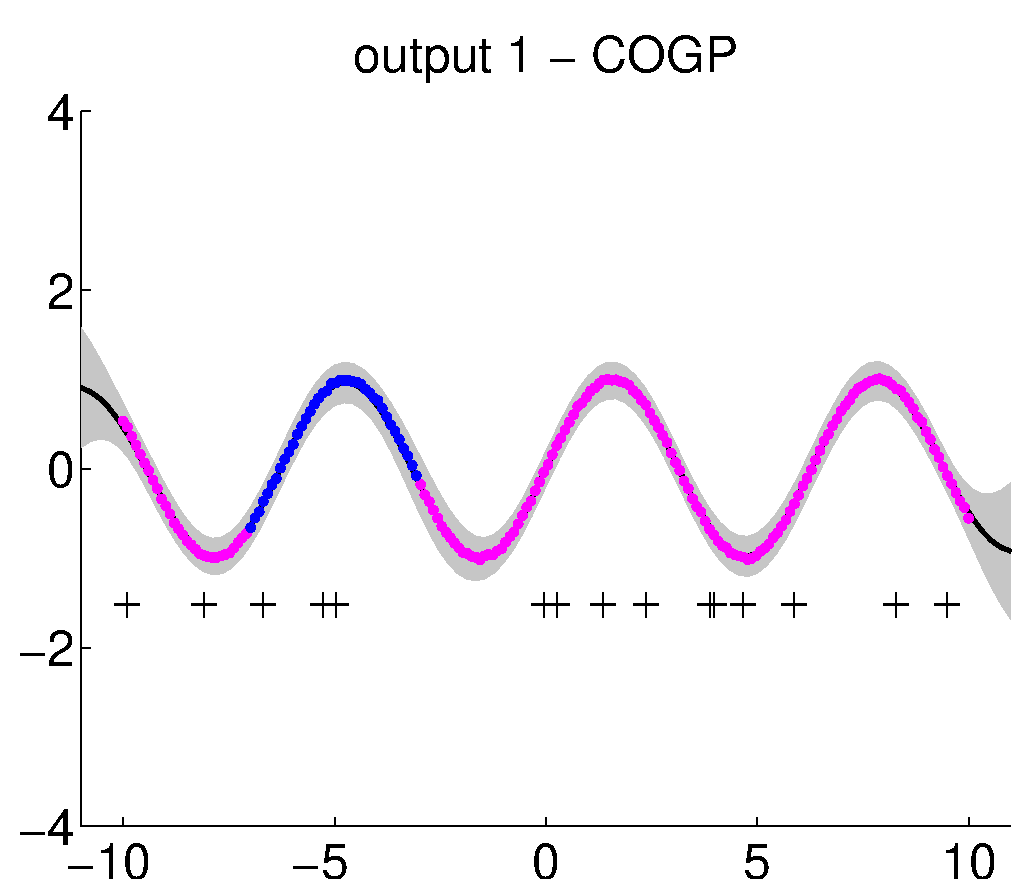
\includegraphics[scale=0.2]{figures/toy-slfm-y1.eps} &
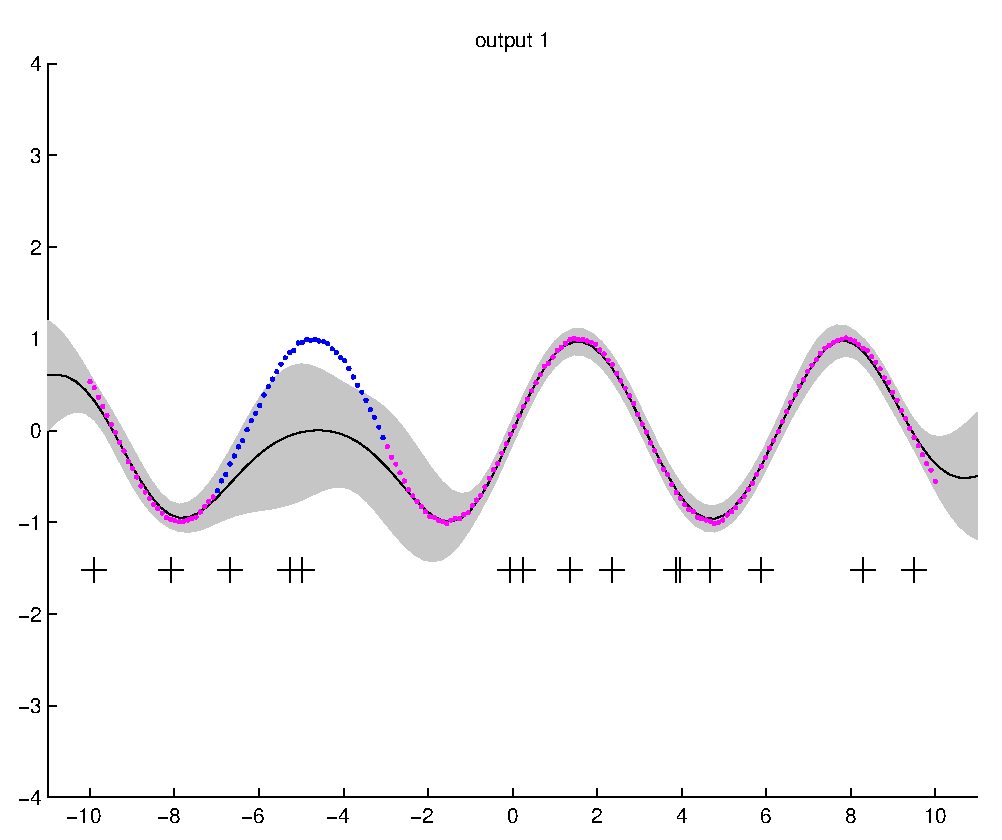
\includegraphics[scale=0.2]{figures/toy-svigp-y1.eps} &
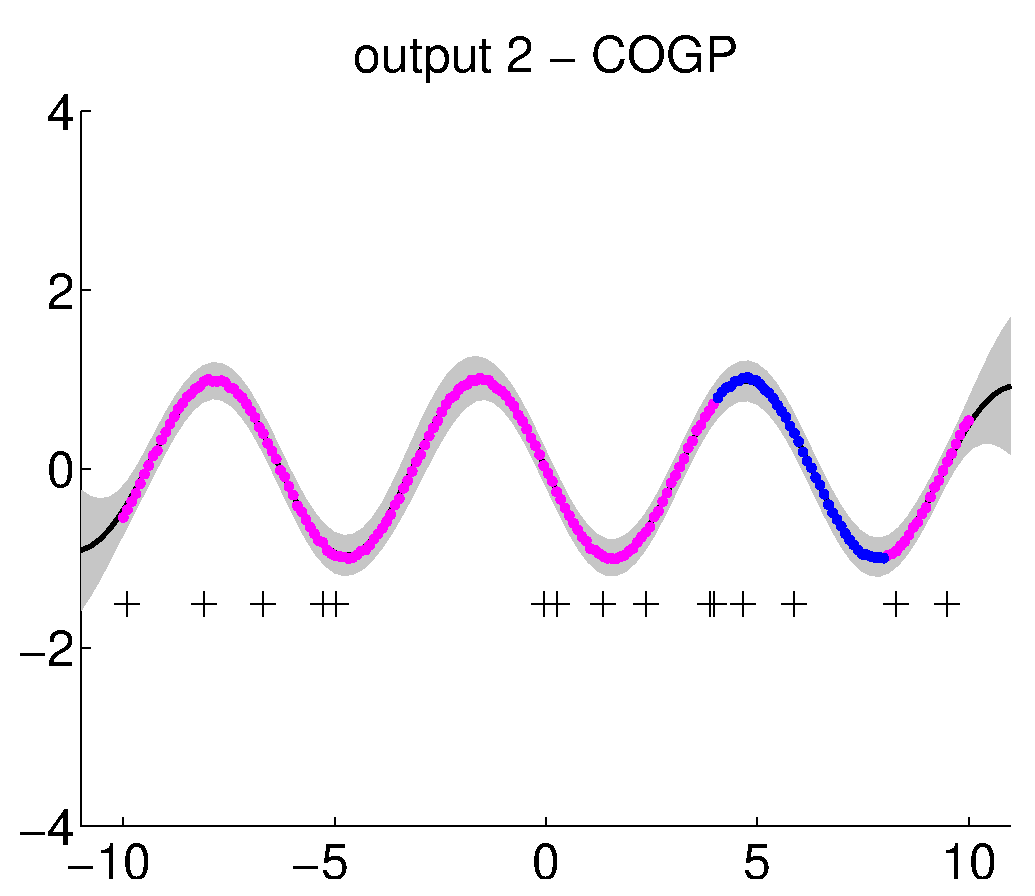
\includegraphics[scale=0.2]{figures/toy-slfm-y2.eps} &
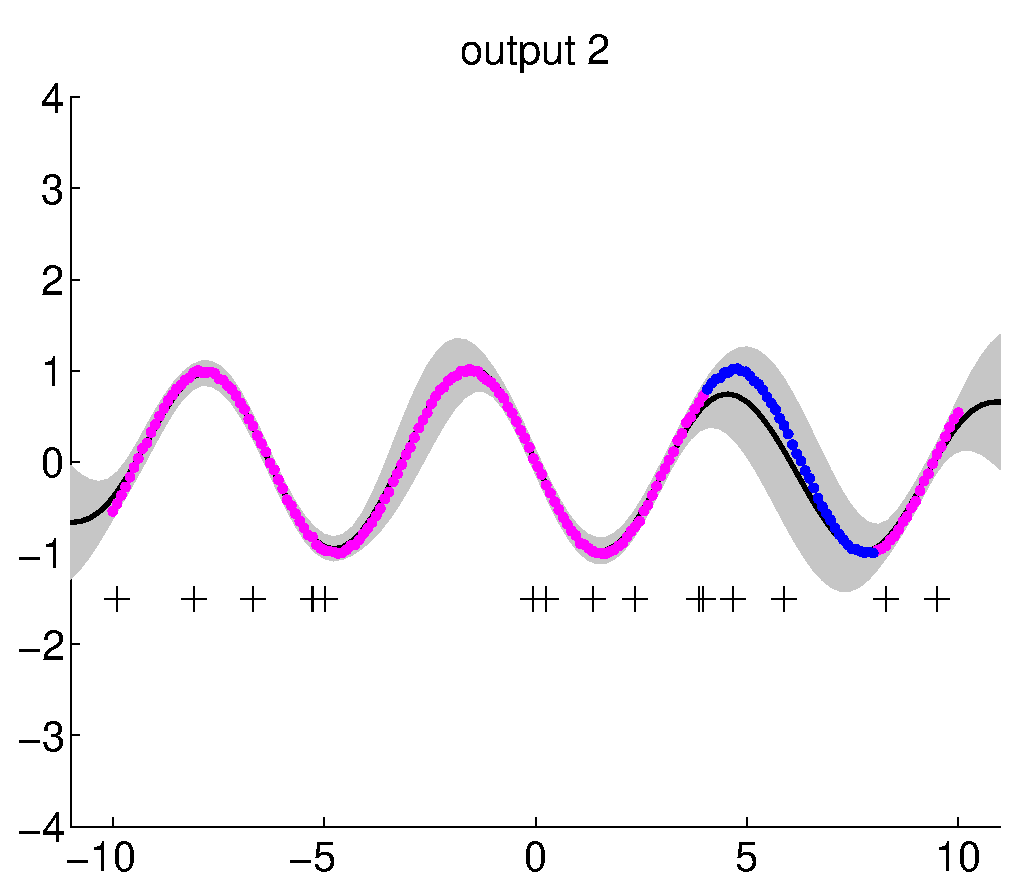
\includegraphics[scale=0.2]{figures/toy-svigp-y2.eps}
\label{fig:toy}
\end{tabular}
\caption{Predictive distributions of the multioutput GPs (first and third figure) and independent GPs using stochastic variational inference (second and last figure) for the  toy problem. Solid black line: predictive mean; grey bar: two standard deviations; magenta dots: real observations; blue dots: missing data. The black crosses show the locations of the inducing inputs.}
\label{fig:toy}
\end{figure*}

\subsection{FOREIGN EXCHANGE RATE PREDICTION}
The application considered here is to predict the foreign exchange rate w.r.t the US dollar of the top 10 international currencies (CAD, EUR, JPY, GBP, CHF, AUD, HKD, NZD, KRW, and MXN) and 3 precious metals (gold, silver, and platinum)\footnote{Data is available at http://fx.sauder.ubc.ca/data.html}. 
The setting of our experiment described here is identical to that in \citet{alvarez2010efficient}.
The dataset contains all the data available for the 251 working days in the year of 2007.
There are 9, 8, and 42 days of missing values  for gold, silver, and platinum, respectively.
We remove from the data the exchange rate of CAD on days 50-100, JPY on day 100-150, and AUD on day 150-200.
Note that these 3 currencies are from very different geographical locations. 
The 153 points extracted is used for testing and the remaining 3051 data points is used for training.
Since the missing data is long contiguous sections, the objective is to evaluate the capacity of the model to impute the missing currency values based on other currencies.
%todo: batch size, learn rate (maybe at the beginning of experiments)

For preprocessing we normalized the outputs to have zero mean and unit variance.
Since the exchange rates are driven by a small number of latent market forces \citet{alvarez2010efficient}, we tried different values of $Q = {1,2,3}$ and selected $Q = 2$ which gave the best model evidence (ELBO).
We used the squared-exponential covariance function for the shared processes and a noise covariance function for the independent process of each output.
The inducing inputs $(M = 100)$ are randomly selected from the training set and fixed throughout training.

The predictive distributions by our model (Figure \ref{fig:fx}) exhibit similar behavior to those by the convolved model with inducing kernels in \citet{alvarez2010efficient}.
In particular, both models perform better at capturing the strong depreciation of the AUD than the fluctuations of the CAD and JPY currency.
Our investigation of the dataset found that 4 other currencies (GBP, NZD, KRW, MXN) also experienced the same trend during the days 150 - 200.
This was effectively used by the model to extrapolate the values of the AUD.

%todo: result for independent gps
We also report in Table \ref{tab:fx} the predictive accuracy of our model compared to the convolved GPs model with exact inference \citet{alvarez-lawrence-nips-08} (CGP) and with approximation via the variational inducing kernels \citet{alvarez2010efficient}) (CGPVAR) in addition to using independent GPs (IGP, one for each output).
Our model outperforms both of the CGP variants in terms of standardized mean-squared error (SMSE).
It has lower test likelihood, as measured by the negative log predictive density (NLPD), which is mainly due to the less conservative predictive variance of the exact CGP for the CAD currency.
The results are averaged across the 3 outputs over 5 repetitions.
% no std because there are 3 outputs but variance is small
Note that the SMSE of CGPVAR is taken from \citet{alvarez2010efficient} while the NLPD was not provided.
Training took only 10 minutes for our model compared to 1.4 hours of the full CGP model.

\begin{table}[h]
\caption{Performance comparison on the foreign exchange rate dataset.}
\label{tab:fx}
\begin{center}
\begin{tabular}{c|c|c}
METHOD & SMSE & NLPD \\ \hline
COGP  & \textbf{0.2125} & -0.8394 \\
CGP & 0.2427 & \textbf{-2.9474} \\
IGP & 0.5996 & 0.4082 \\
CGPVAR & 0.2795 & NA 
%ICM & 0.3927 &
\end{tabular}
\end{center}
\end{table}

\begin{figure*}
\centering
\begin{tabular}{ccc}
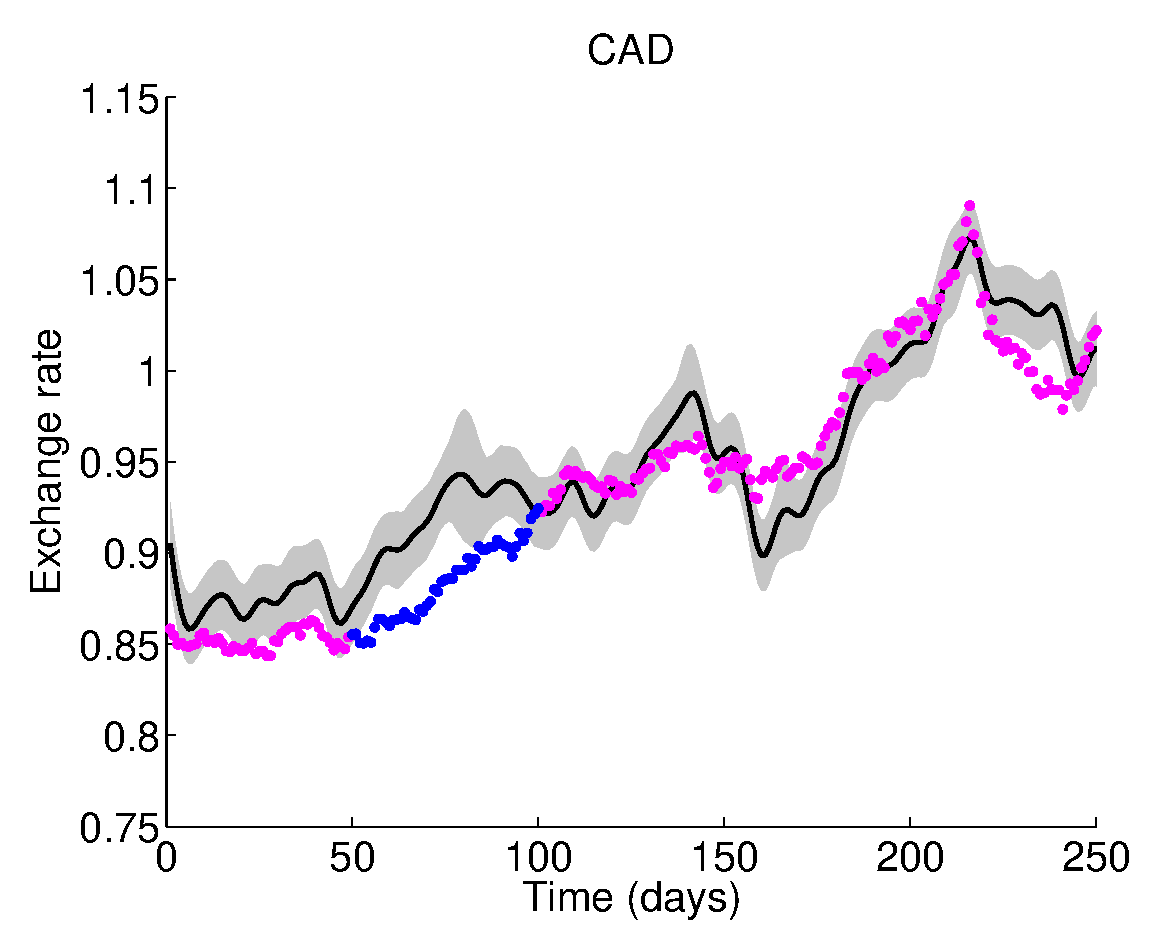
\includegraphics[scale=0.3]{figures/fxCAD.eps} &
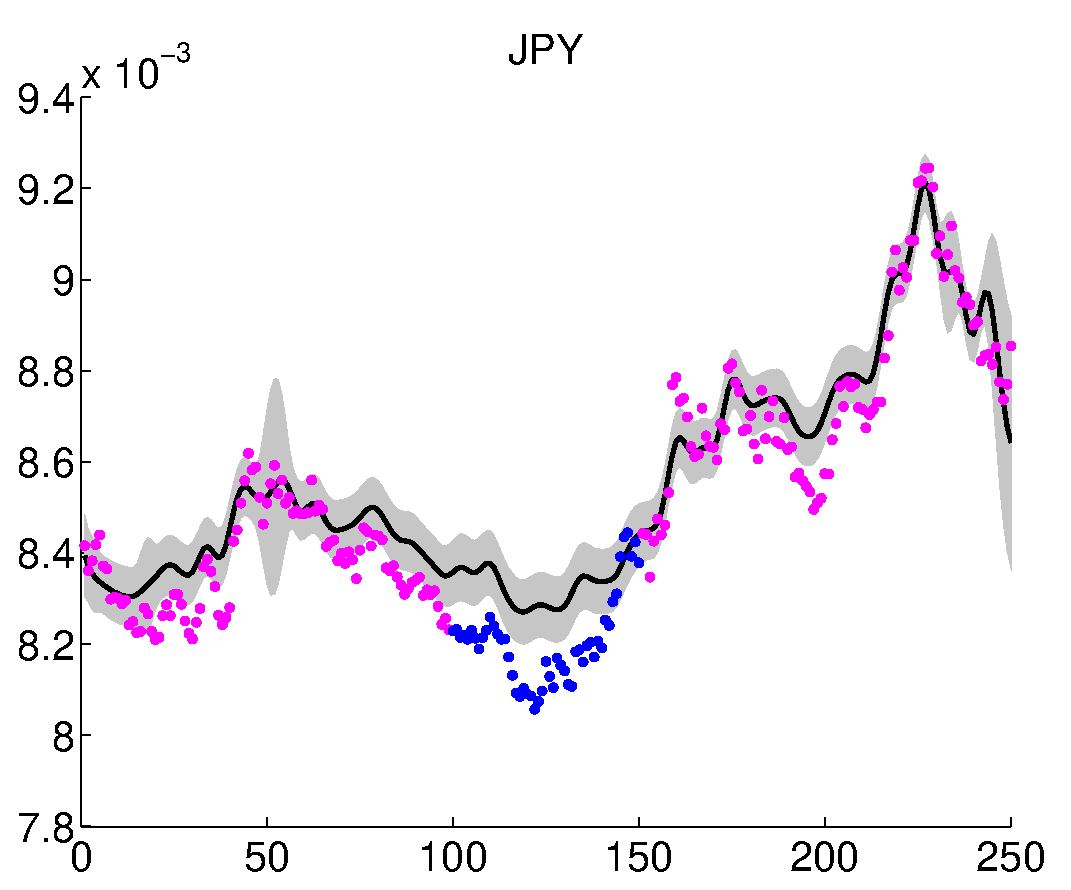
\includegraphics[scale=0.3]{figures/fxJPY.eps} &
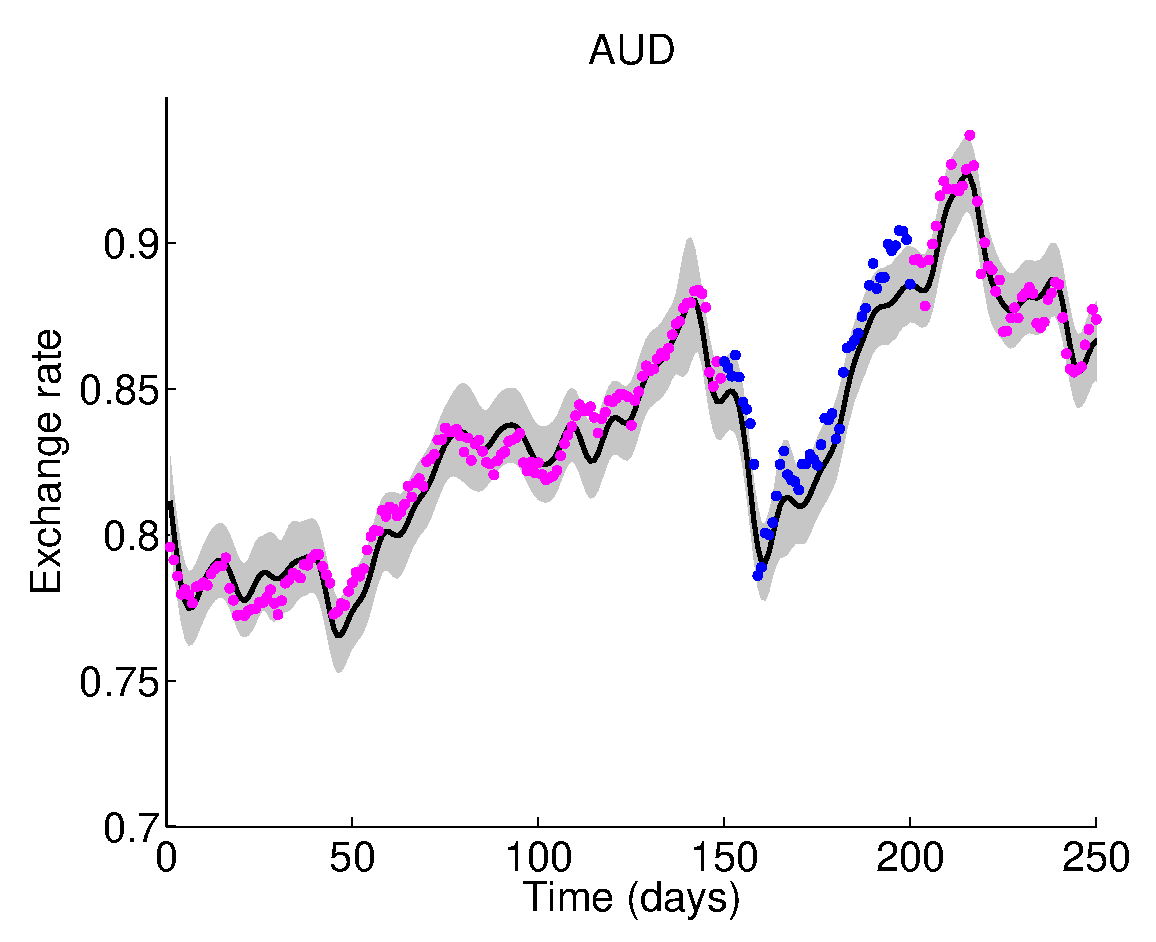
\includegraphics[scale=0.3]{figures/fxAUD.eps}
\end{tabular}
\caption{Real observations and predictive distributions for CAD (left), JPY (middle), and AUD (right). The color coding scheme is the same as in figure \ref{fig:toy}.}
\label{fig:fx}
\end{figure*}

\subsection{AIR TEMPERATURE PREDICTION}
Next, we consider the task of predicting air temperature at 4 different locations in the south coast of England. 
The data is gathered from a network of weather sensors (named Bramblemet, Sotonmet, Cambermet, and Chimet), each of which measures several environmental variables \citet{osborne2008towards}\footnote{Data is available at seperate web pages, see e.g. http://www.bramblemet.co.uk}.
%The sensors are close geographically so we can expect correlation in air temperature.
We selected the sensor signal for air temperature during the period from July 10 to July 15, 2013.
The sensors record measurements every 5 minutes, resulting in a maximum of 4320 observations.
However, there are missing data for Bramblemet (100 points), Chimet (15 points), and Sotonmet (1002 points), possibly due to network outages or hardware failures.
We further simulated failure of the sensors by removing the observations from the time periods [10.2 - 10.8] for Cambermet and [13.5 - 14.2] for Chimet.
The removed data comprises 375 data points, which is used for testing, and the remaining data consisting of 15,788 points is used for training.
Similar to the previous experiment, the objective is to evaluate the ability of the model to use the signals from the functioning sensors to extrapolate the missing signals.

For pre-processing we normalized the outputs to have zero mean and unit variance.
The inducing inputs $(M = 200)$ are randomly selected from the training set and fixed throughout training.
The number of latent processes is $Q = 2$ for both our model and the CGP model.

The real data and the predictive distributions by 3 models (COGP, CGP with exact inference, and independent GPs) are shown in Figure \ref{fig:weather}.
It is clear that the independent GPs model is clueless in the test regions and thus simply uses the average temperature as its prediction.
For Cambermet, both COGP and CGP can capture the rising in temperature from the morning till the afternoon and the fall afterward.
For Chimet, both models perform poorly but CGP more so as it falsely predicts  wild fluctuations that are non-existent in the data. 
Note that the two latent processes learned by our model indeed correspond to different patterns in the data: one process has the inverse lengthscale of 136 which captures the global increase in temperature during the training period while the other has the inverse lengthscale of 0.5 to model the local variations within a single day.
The comparative performance of the models are summarized in Table \ref{tab:air}, which further supports the qualitative analysis that our model outperforms CGP.
All results are averaged of the 2 outputs over 5 repetitions.
Training of our model took on average 5 minutes compared to 3 hours of CGP with exact inference.

\begin{table}[h]
\caption{Performance comparison on the air temperature dataset.}
\label{tab:air}
\begin{center}
\begin{tabular}{c|c|c}
METHOD & SMSE & NLPD \\ \hline
COGP & \textbf{0.1077} & \textbf{2.1712} \\
CGP & 0.1125 & 2.2219 \\
IGP & 0.8944 & 12.5319
\end{tabular}
\end{center}
\end{table}

\begin{figure*}
\centering
\begin{tabular}{ccc}
\includegraphics[scale=0.3]{figures/slfm-weatherCambermet.eps} &
\includegraphics[scale=0.3]{figures/cgp-weatherCambermet.eps} &
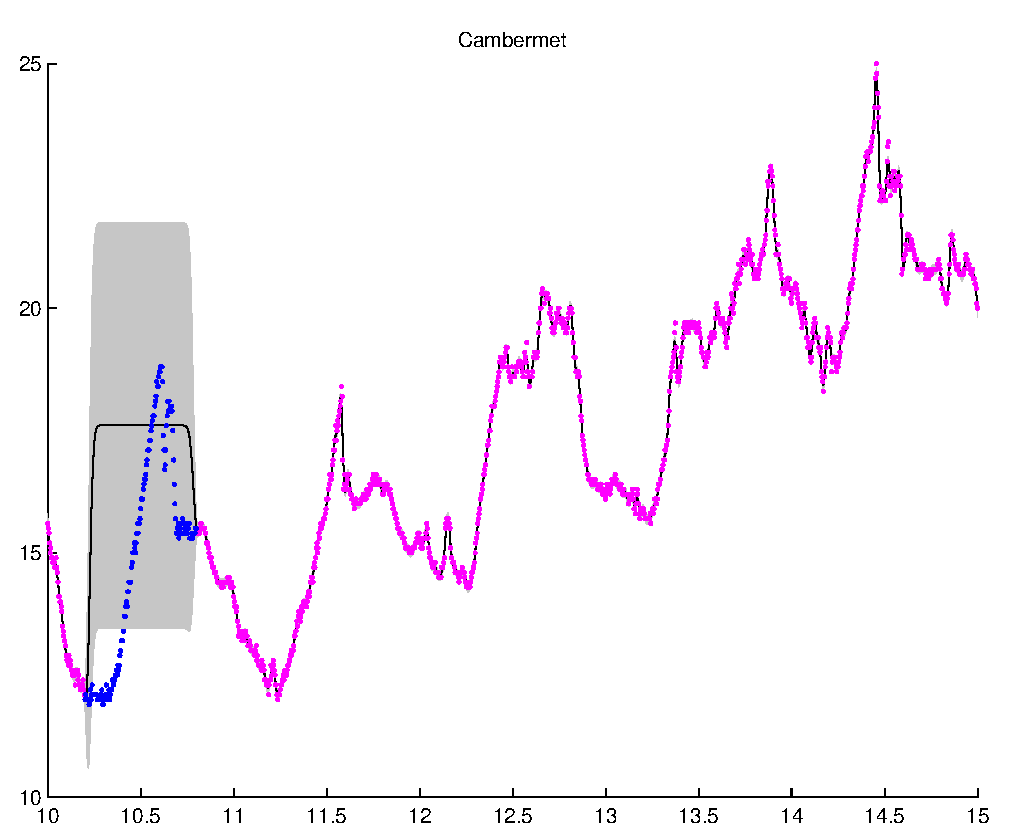
\includegraphics[scale=0.3]{figures/weatherCambermet.eps}
\\
\includegraphics[scale=0.3]{figures/slfm-weatherChimet.eps} &
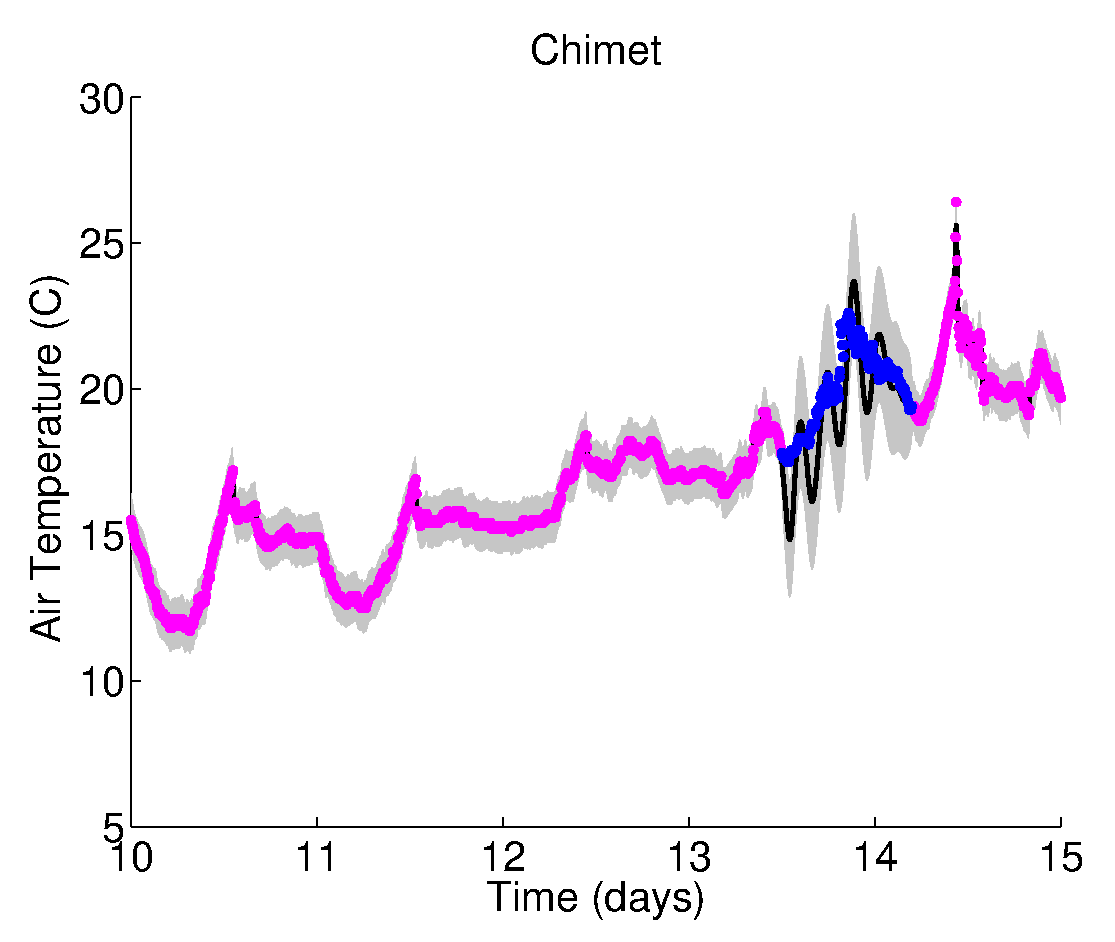
\includegraphics[scale=0.3]{figures/cgp-weatherChimet.eps} &
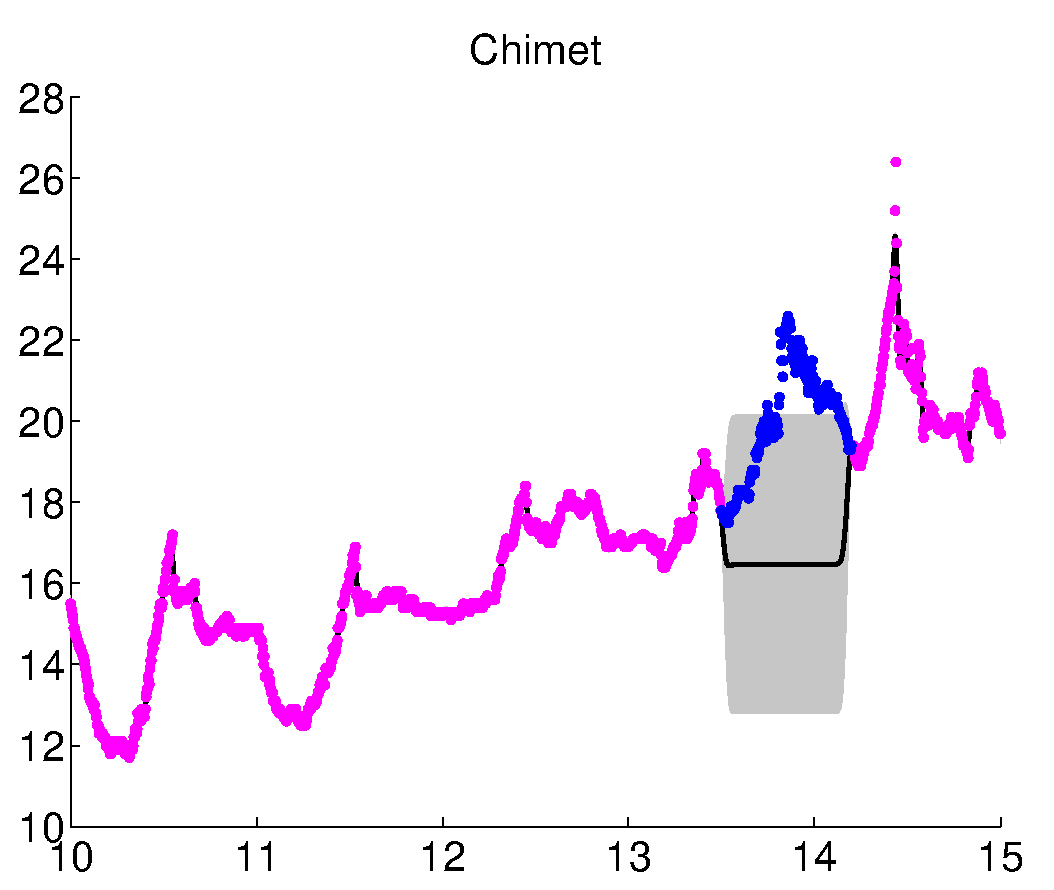
\includegraphics[scale=0.3]{figures/weatherChimet.eps}
\end{tabular}
\caption{Predictive distributions of the multioutput GPs (left column) and full independent GPs (right column) for the air temperature problem.}
\label{fig:weather}
\end{figure*}

\subsection{ROBOT ARMS}


\section{DISCUSSION \label{sec:discussion}}
We have presented scalable multi-output GPs for learning of correlated functions.
The formulation around the inducing variables and their encapsulation of sufficient statistics was shown to be conducive to not only effective but also scalable joint learning under sparsity. 
We note that although our large scale experiment was done with over 40,000 observations -- the largest publicly available multi-output dataset we could find, the model can easily handle much bigger datasets.

We discuss several interesting extensions to this work.
First, consider the model for the single GP case, i.e., $P = 1$. By using $Q > 1$ sparse processes, the GP can now have multiple set of inducing variables.
These can be made local to capture varying characteristics of the latent process in different  input regions, for e.g. similar to the 
work by \citet{nguyen2014fast}, leading to scalable GPs with non-stationary properties. 

A further extension is to replace the constant mixing weights in the model with input-dependent coefficients as in the Gaussian process regression networks framework \citep[GPRN,][]{wilson-et-al-icml-12} to accommodate adaptive dependencies among the outputs.
We leave  these extensions to future work.

%\subsubsection*{Acknowledgements}

\bibliographystyle{apalike}
\bibliography{references}

\end{document}
